\section{WMod - Wide-Angle High-Mach Modal Code}

{\bf WMod} implements a normal mode expansion for propagation of a single tone in a stratified atmosphere. In contrast to {\bf Modess}, {\bf Wmod} does not use the effective sound speed approximation but rather treats the background wind rigorously in the planar (2-d) approximation, with the assumption that vertical wind shear is small over the scale of a wavelength and can thus be neglected. Since it does not use the effective sound speed approximation, {\bf WMod} can accurately model the high propagation angles required for long range propagation that depends on refraction from the upper atmosphere and can, in principle, be used to model propagation under conditions of arbitrarily high background wind speeds. {\bf WMod} represents a significant improvement over {\bf Modess}; however, computation times are much longer. As in {\bf Modess}, atmospheric attenuation in {\bf Wmod} is taken into account using first order perturbation theory. More details can be found in \cite{assink_dissertation}.

\subsection{Mathematical Background}
\label{sec: wmod math}
As in section~\ref{sec: modess math} let $z$ denote altitude above the ground surface and let the subscript $H$ denote horizontal displacement. Let $r=\|\textbf{x}_{H}\|$ be the radial horizontal range. Let $\rho_0$ be the mean density of the atmosphere, let $\alpha$ be the atmospheric attenuation coefficient, $\omega$ the angular frequency, and $p$ the deviation from mean pressure at horizontal position $\textbf{x}_{H}$ and altitude $z$. Then {\bf WMod} solves the following generalized Helmholtz equation: 
\begin{equation}
\Big[ 
\nabla_{H}^2 
+ 
\rho_0 \frac{\partial}{\partial z} \Big(\frac{1}{\rho_0} \frac{\partial}{\partial z} \Big) 
+
\Big(\frac{\omega}{c(z)}+ i\frac{\textbf{v}_{0,H}}{c(z)} \cdot \nabla_{H}+i\alpha(\omega,z)\Big)^2 
\Big] \hat{p}_A(r,z,\omega) = 0.
\label{eq: full planar Helmholtz}
\end{equation}
The pressure deviation $p$ satisfies the boundary condition 
\[
\frac {\partial p}{\partial z}\Big |_{z=0}= 0
\]
on the ground surface. If the signal source is assumed to be at zero range, $r=0$, and altitude $z_S$ then $p$ is asymptotic, for small distance $r,(z-z_S)\downarrow 0$, to the field produced by a unit acoustic source, 
\[
\lim_{r,(z-z_S)\downarrow0}\Big(p(r,z,\omega)-\frac{1}{\sqrt{r^2+(z-z_S)^2}}\Big)=0.
\]

As for {\bf Modess}, the solution is again obtained by the method of normal modes. Computed is the modal sum for the far field pressure deviation 
\[
p(r,z,\omega)
\approx
\frac{e^{i \pi /4}}{\sqrt{8 \pi r}} \sqrt{\frac {\rho_0(z)} {\rho_0(z_s)}} \sum_j\psi_j(z_s)\psi_j(z) \frac{e^{i (k_j+i\alpha_j)r}}{\sqrt{k_j}},
\]
precisely as in equation~\ref{eq: modess far field pressure}. As for {\bf Modess} the modal wave numbers $k_j$ and mode functions $\psi_j$ are real valued; however, $k_j$ (rather than $k_j^2$) are now the eigenvalues and $\psi_j$ the corresponding eigenfunctions of the quadratic (since $k$ appears quadratically) eigenvalue problem 
\[
\Big( 
\frac{d^2}{dz^2} +\frac{\omega^2}{c^2}
\Big)\psi(z) 
= 
\Big((1-\nu^2)k^2+2\nu\frac{\omega}{c}k\Big)\psi(z) 
\quad \text{with} \quad 
\psi^\prime(0)=0 
\]
where, for $\hat{\textbf{k}}_{H}$ the unit vector in the horizontal direction of propagation, $\nu=\hat{\textbf{k}}_{H}\cdot\frac{\textbf{v}_{0,H}}{c}$. The modal attenuation coefficients are estimated perturbatively as in section~\ref{sec: modess math}. 

The eigenvalue problem is solved as in section~\ref{sec: modess math} by replacing the continuous vertical domain with a uniformly spaced discrete grid, using finite differences to approximate the derivatives with respect to $z$, truncating the vertical domain at some large altitude, T, and then solving the resulting finite dimensional eigenvalue problem. Using the notation introduced in section~\ref{sec: modess math} the eigenvalue problem reduces to a large dimensional linear algebra problem: find the eigenvalues $k$ and corresponding eigenvectors $\Psi$ that satisfy 
\[
M\Psi=Ak^2\Psi+Bk\Psi
\]
where $A$ and $B$ are diagonal matrices with entries in the $n,n$ position given by $1-\nu(nh)^2$ and $2\nu(nh)\frac{\omega}{c(nh)}$ respectively. 

As with the effective sound speed approximation, only a small subset of the set of the eigenvalues is required; however, determining the relevant range of eigenvalues is not as straightforward for the quadratic eigenvalue problem being considered here as it is for the linear eigenvalue problem associated with the effective sound speed. In practice, it has been found sufficient for the relevant phase velocities to be chosen as in the effective soundspeed case, as depicted in Fig.\,\ref{fig:wvnums_modess}. Once the range of phase velocities has been determined, the eigenvalues and corresponding mode functions are computed using the quadratic eigenvalue solver contained in the \textbf{SLEPc} package. 


\subsection{Running WMod}
\label{sec:running wmod}

Making sure that the executable for {\bf Wmod} is in the system's path, it can be run by entering 
\begin{verbatim} 
    WMod [--option1 val1] [--option2 val2] [...] [--flag1] [...] 
\end{verbatim}
on a command line. Generally, options are followed by values, either numbers, strings or filenames. Flags are not. Entering \verb"WMod --help" sends the following help page to the screen: 

\begin{verbatim}
By default the program computes the 1D transmission loss (TL) at the ground or
the specified receiver height and saves the data to 2 files:
    file wtloss_1d.nm - considering attenuation in the atmosphere
    file wtloss_1d.lossless.nm - no attenuation
Additionally, if the flag --write_2d_tloss is present on the command line, the
2D TL is saved to file wtloss2d.nm. The user can also choose to propagate in N
different directions i.e. (N by 2D mode) by using the option --multiprop.

The options below can be specified in a colon-separated file "wmod.param" or at
the command line. Command-line options override file options.

Options Control:
  -h, --help             Prints help test
  --paramfile            Parameter file name [modess.param]
  --printparams          Print parameter summary to screen

Required Parameters:
  --atmosfile            Atmospheric profile filename
  --freq                 Frequency of analysis (Hz)

Optional Parameters [default]:
  --maxheight_km         Maximum height of analysis in km [150.0]
  --zground_km           Ground height [take from Z0 parameter in atmosfile, or
                         0.0]
  --Nz_grid              Number of vertical grid points to use [20000]
  --sourceheight_km      Source height in km [0.0]
  --receiverheight_km    Receiver height in km [0.0]
  --maxrange_km          Maximum range in km to use for modeling [1000.0]
  --Nrng_steps           Number of range steps to use [1000]
  --ground_impedence_model
                         Impedence model to use. Currently only "rigid" is
                         supported. [rigid]
  --use_attn_file        File name containing attenuation, to override default
                         Sutherland/Bass [n/a]. Columns are
                         Height(km) Attenuation(np/m)
  --dispersion_file      Filename to output the dispersion information
    --append_dispersion_file
                         Append results to dispersion file rather than
                         overwriting

Modes of Operation:
  --singleprop           Single azimuth propagation. Requires --azimuth
    --azimuth            Azimuth of propagation, in degrees CW from North
                         [0,360)
  --multiprop            Multiple azimuth propagation. Requires --azimuth_start,
                         --azimuth_end, and --azimuth_step
    --azimuth_start      Starting azimuth, in degrees CW from North [0,360)
    --azimuth_end        Ending azimuth, in degrees CW from North [0,360)
    --azimuth_step       Azimuth step, in degrees CW from North [0,360)

Flags:
  --write_2d_tloss       Output 2-D transmission loss to tloss2D.nm
  --write_phase_speeds   Output phase speeds to phasespeeds.nm
  --write_modes          Output modes to mode_###.nm. Also implies
                         --write_speeds
  --write_atm_profile    Output atmospheric profile to atm_profile.nm
  --Lamb_wave_BC         Use admittance = -1/2*dln(rho)/dz
  --turnoff_WKB          Turn off the WKB least phase speed estimation
  --wvnum_filter         Use wavenumber filter by phase speed. Requires --c_min
                         and --c_max
    --c_min              Minimum phase speed to keep
    --c_max              Maximum phase speed to keep



OUTPUT Files: Format description (column order):
  wtloss_1d.nm:                 r, 4*PI*Re(P), 4*PI*Im(P), (incoherent TL)
  wtloss_1d.lossless.nm:
  wtloss_2d.nm:                 r, z, 4*PI*Re(P), 4*PI*Im(P)
  Nby2D_wtloss_1d.nm:
  Nby2D_wtloss_1d.lossless.nm:  r, theta, 4*PI*Re(P), 4*PI*Im(P), (incoherent TL)
  wphasespeeds.nm:              Mode#, phase speed [m/s], imag(k)
  wmode_<mode_count>.nm         z, (Mode amplitude)
  wdispersion_<freq>.nm         Contains one line with entries:
                               freq, (# of modes), rho(z_src), rho(z_rcv)
                               followed for each mode 'i' by quadruples:
                               real(k(i)), imag(k(i)), Mode(i)(z_src), Mode(i)(z_rcv)
  atm_profile.nm               z,u,v,w,t,d,p,c,c_eff

Examples (run from 'samples' directory):
    ../bin/WMod --singleprop --atmosfile profile_noheader.dat \
         --atmosheaderfile sampleheader.dat --azimuth 90 --freq 0.1

    ../bin/WMod --singleprop --atmosfile NCPA_canonical_profile_zuvwtdp.dat \
         --azimuth 90 --freq 0.1 --write_2d_tloss --sourceheight_km 60 \
         --receiverheight_km 60

    ../bin/WMod --multiprop --atmosfile NCPA_canonical_profile_zuvwtdp.dat \
         --freq 0.1 --azimuth_start 0 --azimuth_end 360 --azimuth_step 1

\end{verbatim}

The options and flags for {\bf WMod} are the same as for {\bf Modess}. The reader is referred to the {\bf Modess} documentation above for explanations. The only difference is that the output filenames now have a \verb+w+ preceding \verb+tloss+ in each case. 


\subsection{Running WMod: examples}
\label{sec: wmod examples}

The \textbf{WMod} help page ends with three examples. The examples set the frequency to 0.1 Hz to keep run times short. The first is a simple example illustrating the primary input modes for \textbf{WMod}. It is assumed that the user runs it in the \verb+samples+ directory. Note that if the \textbf{ncpaprop} \verb+bin+ directory is in the system's path one may enter \verb+WMod+ rather than \verb+../bin/WMod+. The command line entry for the example is 
\begin{verbatim} 
    ../bin/WMod --singleprop --atmosfile profile_noheader.dat \
         --atmosheaderfile sampleheader.dat --azimuth 90 --freq 0.1
\end{verbatim}
In this example the four required options are set, and an external header file is specified. Otherwise the default settings are used. Ground-to-ground propagation in the NCPA toy atmosphere (see Figure \ref{fig:canonic_sound_speeds}) at 90 degrees azimuth (from North), eastward propagation, at frequency of 0.1 Hz is modelled. By default the signal is propagated out to 1000 km in range with range steps of 1 km. The atmospheric profiles are specified in the column-based text file \verb"profile_noheader.dat" that is included in the \verb+samples+ directory, and the profile metadata is provided in the additional text file \verb"sampleheader.dat" rather than as a header in the same file. 

\begin{figure}
\begin{center}
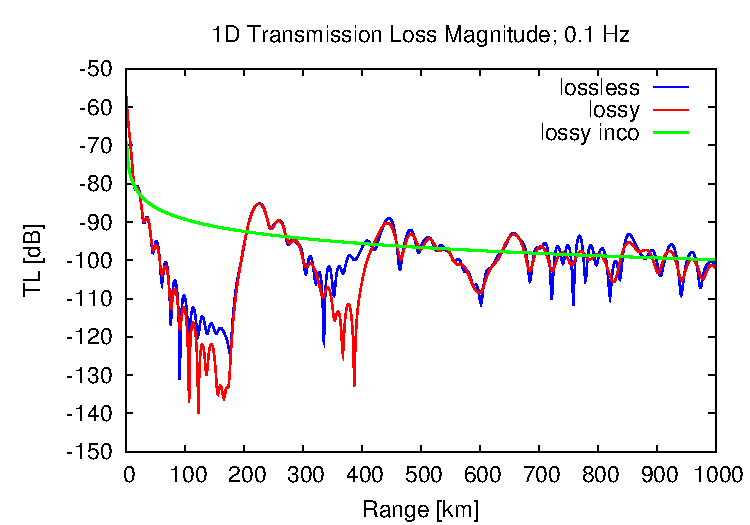
\includegraphics[scale=0.60]{figs/modess_ex1}
\end{center}
\caption{1D transmission loss magnitude at 0.1 Hz obtained with \textbf{WMod} for eastward ground-to-ground propagation in the NCPA toy atmosphere shown in Figure \ref{fig:canonic_sound_speeds}. Shown are the lossless transmission loss magnitude, the lossy transmission loss magnitude and the lossy incoherent transmission loss.}
\label{fig: wmod 1D tl}
\end{figure}

The output is, by default, the one-dimensional (1D) transmission loss on the ground for both lossy and lossless cases and is written into the text files \verb+wtloss_1d.nm+ and \verb+wtloss_1d.lossless.nm+ as described above in the \verb+WMod+ help page; see section~\ref{sec:running wmod} and section~\ref{sec:running modess} for more discussion.  An example of the magnitude of the complex 1D transmission loss output is shown in Figure \ref{fig: wmod 1D tl}. Note that in general the output from all programs will be saved in the directory from which the code is run.  

\begin{figure}
\begin{center}
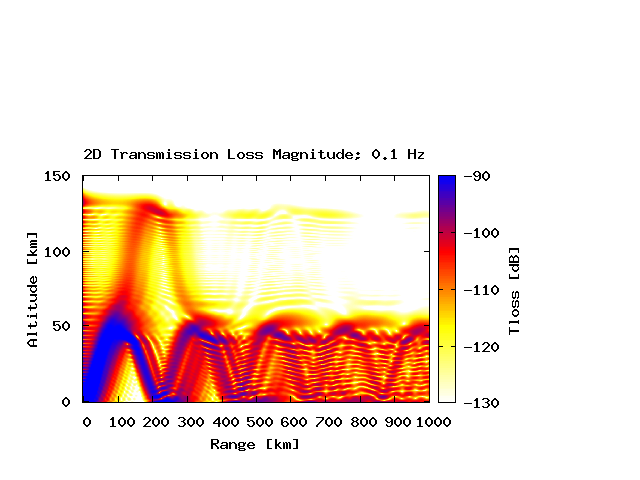
\includegraphics[scale=0.45,trim = 20 20 110 140,clip]{figs/wmod_ex2}
\end{center}
\caption{2D transmission loss magnitude at 0.1 Hz obtained with {\bf WMod} for eastward propagation in the NCPA toy model. The source is placed on the ground at the origin.}
\label{fig: wmod 2D tl}
\end{figure}

\newpage

In the second example the \verb+--write_2D_Tloss+ flag is appended to the command line entry for the first example: 
\begin{verbatim} 
    ../bin/WMod --singleprop --atmosfile NCPA_canonical_profile_zuvwtdp.dat \ 
                --azimuth 90 --freq 0.1 --write_2d_tloss
\end{verbatim}
As described above and in section~\ref{sec:running modess}, the output is written to a default file, in this case \verb+wtloss2d.nm+. The 2D transmission loss magnitude that results from eastward propagation in the NCPA toy model is plotted in Figure \ref{fig: wmod 2D tl}.  In the above example the profile file has 7 columns in the order \verb"zuvwtdp" (refer to section~\ref{sec: AtmoSpecs}  for an explanation of atmospheric specifications).

\begin{figure}[h]
\begin{center}
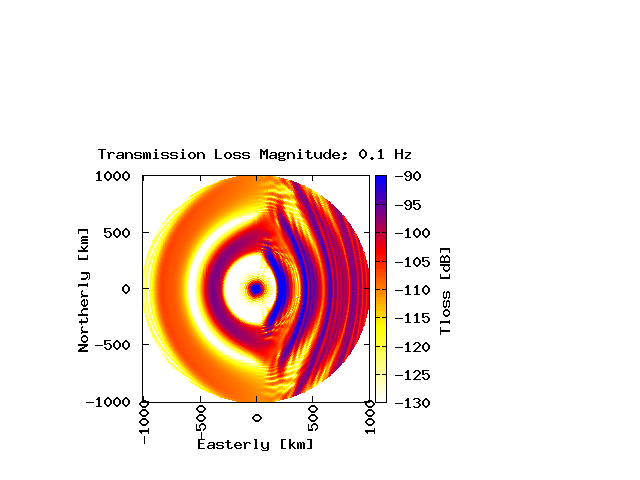
\includegraphics[scale=0.45,trim = 70 20 180 140,clip]{figs/wmod_ex3}
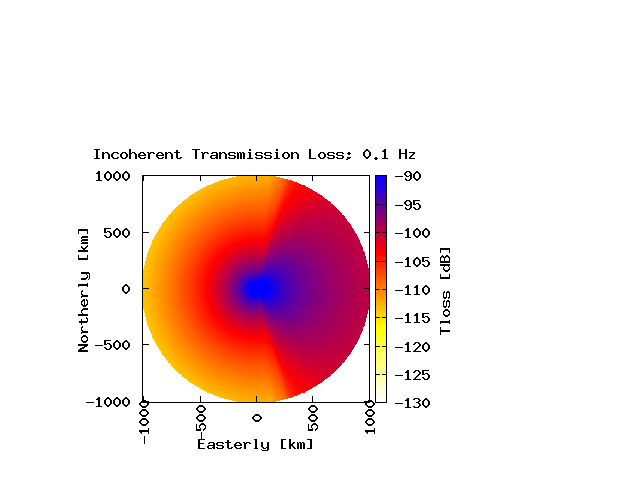
\includegraphics[scale=0.45,trim = 70 20 180 140,clip]{figs/wmod_ex3_inco}
\end{center}
\caption{N by 2D transmission loss magnitude and incoherent transmission loss obtained with {\bf WMod} for ground-to-ground propagation in the NCPA toy model atmosphere from a source at the origin to all azimuths.}
\label{fig: wmod Nby2D tl}
\end{figure}

In the third example the \verb+--multiprop+ flag is appended to the command line entry for the first example. This flag requires that values for the options \verb+--azimuth_start+, \verb+--azimuth_end+, and \verb+--azimuth_step+ be given. 
\begin{verbatim} 
    ../bin/WMod --multiprop --atmosfile NCPA_canonical_profile_zuvwtdp.dat \
                --freq 0.1 --azimuth_start 0 --azimuth_end 360 --azimuth_step 1
\end{verbatim}
The output is written to the files \verb+Nby2D_wtloss_1d.nm+ and \verb+Nby2D_wtloss_1d.lossless.nm+ as described above in section~\ref{sec:running wmod}. The lossless transmission losses are also computed and saved as are the incoherent transmission losses and the resulting transmission loss magnitude is plotted in Figure \ref{fig: wmod Nby2D tl}. 
